\chapter{Findings So Far}
\label{ca:chap:findings}

All three hypotheses have now been run once at full scale, with three seeds. This chapter
reports what we have found and how confident each finding is.

\section{Text-Only Supervision Avoids the Tokenizer Cost}
\label{ca:sec:motivating}

The black-box assumption gives up the teacher's token probabilities. To see what those are
worth, we ran on-policy distillation from Qwen3-4B-Instruct on Countdown with three
students, each first fine-tuned to the same starting accuracy of about 0.38
(Table~\ref{ca:tab:motivating}). Recovery $R$ is the fraction of the gap between that
starting point and the teacher (0.713) that distillation closed.

\begin{table}[htbp]
\centering
\small
\begin{tabular}{@{}llllc@{}}
\toprule
\textbf{Student} & \textbf{Tokenizer} & \textbf{Loss} & \textbf{Accuracy} & $R$ \\
\midrule
Qwen2.5-1.5B & shared    & exact logits (GKD)         & 0.379 $\to$ 0.600 & 0.66 \\
Qwen2.5-1.5B & shared    & cross-tokenizer loss (ULD) & 0.379 $\to$ 0.487 & 0.32 \\
OLMo-2-1B    & different & cross-tokenizer loss (ULD) & 0.381 $\to$ 0.426 & 0.14 \\
OLMo-2-1B    & different & GOLD hybrid                & 0.381 $\to$ 0.035 & collapsed \\
SmolLM2-1.7B & different & GOLD hybrid                & 0.375 $\to$ 0.000 & collapsed \\
\bottomrule
\end{tabular}
\caption{Each step away from a shared tokenizer roughly halves what distillation recovers,
and the hybrid cross-tokenizer loss collapses. Countdown, 200 steps, 1,000 test puzzles;
the first OLMo-2 GOLD run was stopped at step 110.}
\label{ca:tab:motivating}
\end{table}

The cross-tokenizer loss alone halved recovery on a shared tokenizer (paired difference
$+0.113$, 95\% interval $[+0.091, +0.136]$), and a real mismatch halved it again. The GOLD
hybrid loss collapsed on both cross-tokenizer students while its value kept falling: it
forced OLMo-2 into the teacher's single-digit number tokens, which broke its arithmetic, and
it let SmolLM2 emit newlines to the length limit.

\begin{takeaway}{Text-Only Supervision Is the Safer Choice}
\label{ca:tk:blackbox}
Logit-level supervision across model families is both lossy and fragile, so a reward
computed from the teacher's text is a sound basis for learning from heterogeneous providers.
\end{takeaway}

\section{Selectors Need Feedback from Realised Gains}
\label{ca:sec:pilot}

We first ran every condition once (seed 0, 14.4 GPU-hours) to test the pipeline. The
original headroom selector, which scored arms by headroom over price alone, made the switch
it predicted before training, from Qwen2.5-3B to Qwen2.5-7B on Countdown once the student
passed an accuracy of about 0.27. It then spent 320 of its 400 rounds on MATH, where the
headroom never shrank because nothing was learned. The original Thompson sampling divided
each noisy gain by its cost before learning, which shrinks the noise of expensive arms
towards zero, and it spent 55\% of its budget on the degraded provider. A five-times-higher
learning rate did not help MATH or code and cut the Countdown gain from $+0.280$ to
$+0.098$. We kept the learning rate, added the learned efficiency to the headroom selector,
and made Thompson sampling apply the price only when choosing.

\begin{takeaway}{Headroom Is Not Enough}
\label{ca:tk:feedback}
A domain can have large headroom and no learnability, so a selector must learn from the
progress it actually observes, and noisy gains must not be divided by cost before they are
averaged.
\end{takeaway}

\section{Price, Not Provider Identity, Decides Value (H1, H2)}
\label{ca:sec:h12}

Figure~\ref{ca:fig:mv} shows the marginal value of every provider on every domain at the
four checkpoints, from all 216 branches.

\begin{figure}[htbp]
\centering
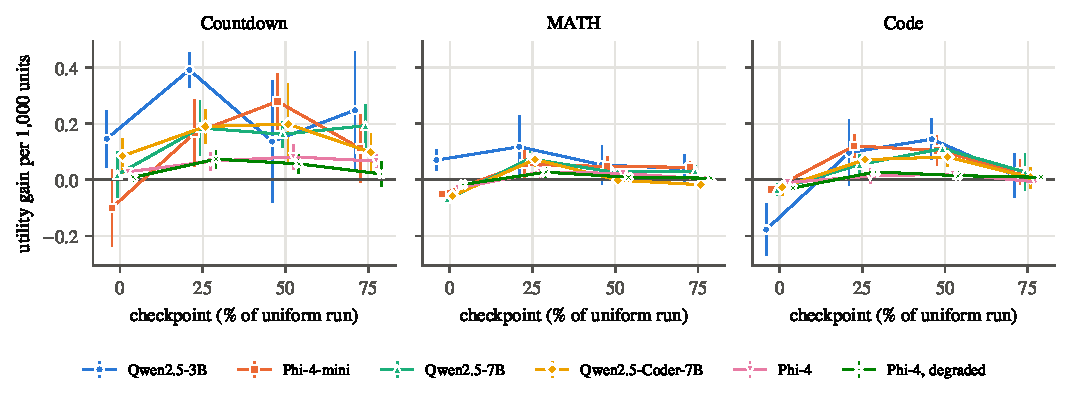
\includegraphics[width=\linewidth]{ca_marginal_value.pdf}
\caption{On Countdown, the cheapest provider usually gives the most progress per unit of
budget, and on MATH and code every provider gives almost none. Change in mean selection
accuracy after 20 rounds on one arm, per 1,000 price units; points are means over three
seeds, bars $\pm 1$ standard error, offset horizontally for legibility.}
\label{ca:fig:mv}
\end{figure}

\paragraph{Cheap providers lead per unit of budget.} On Countdown, the cheapest provider,
Qwen2.5-3B, has the highest mean marginal value at the 0, 25 and 75\% checkpoints, and
Phi-4-mini at 50\%; Qwen2.5-3B is the best Countdown arm in 8 of the 12 combinations of seed
and checkpoint. Per round, without dividing by price, the providers are much closer. For
example, from the 25\% checkpoint all six raise mean utility by between 0.022 and 0.033 in
20 Countdown rounds. Phi-4 teaches no faster per round, to within noise, than providers that
cost a third as much. Its only lead is on code from the untrained student, where every
provider lowered utility and Phi-4 lowered it least. The only differences that are
significant in paired comparisons within a seed all involve Phi-4: at 25\%, Qwen2.5-3B beats
Phi-4 and its degraded copy on Countdown, and Phi-4-mini beats Phi-4 on code.

\begin{takeaway}{Price Decides Value}
\label{ca:tk:price}
Providers of very different strength teach a small student at a similar rate per gradient
step, so value per unit of budget is decided mainly by price, and the strongest provider is
rarely worth its price.
\end{takeaway}

\paragraph{H1 and H2 are below our current resolution.} Our decision rules, fixed before the
runs, require the leading provider's 95\% interval to clear its rival's; here these are
t-intervals over the three seeds. This never happens between the cheap and mid-priced
providers, at any checkpoint or in any domain. The leading provider does change between
checkpoints and domains, and the rankings are unstable: Kendall's $\tau$, which measures how
well the provider ranking at one checkpoint agrees with the ranking at the next, ranges from
$-0.60$ to $0.73$. But changes of that size are also what noise alone would produce.

\begin{takeaway}{H1 and H2 Remain Open}
\label{ca:tk:open}
Among the affordable providers, differences in marginal value are smaller than three seeds
of 20-round branches can detect, so we can neither confirm nor reject that the best
provider differs by domain or changes during training.
\end{takeaway}

\section{Adaptive Selection Matches the Best Provider (H3)}
\label{ca:sec:h3}

Table~\ref{ca:tab:h3} reports every condition on the test set.

\begin{table}[htbp]
\centering
\footnotesize
\setlength{\tabcolsep}{2.5pt}
\begin{tabular}{@{}lrccccc@{}}
\toprule
 & & \multicolumn{3}{c}{\textbf{Test accuracy}} & & \\
\cmidrule(l){3-5}
\textbf{Condition} & \textbf{Rounds} & \textbf{Countdown} & \textbf{MATH} & \textbf{Code} & \textbf{Utility [95\% CI]} & \textbf{Diff. [95\% CI]} \\
\midrule
Untrained student & -- & 0.218 & 0.434 & 0.336 & 0.329 & \\
\midrule
Qwen2.5-3B only & 400 & 0.555 & 0.418 & 0.352 & 0.442 [0.416, 0.468] & $-$0.052 [$-$0.083, $-$0.024] \\
Phi-4-mini only & 400 & 0.630 & 0.438 & 0.352 & 0.473 [0.440, 0.508] & $-$0.020 [$-$0.049, +0.009] \\
Qwen2.5-7B only & 364 & 0.698 & 0.423 & 0.360 & 0.494 [0.468, 0.519] & -- \\
Qwen-Coder-7B only & 360 & 0.656 & 0.421 & 0.358 & 0.478 [0.450, 0.507] & $-$0.015 [$-$0.032, +0.000] \\
Phi-4 only & 110 & 0.417 & 0.429 & 0.335 & 0.394 [0.370, 0.417] & $-$0.100 [$-$0.127, $-$0.073] \\
\midrule
Uniform & 223 & 0.556 & 0.437 & 0.343 & 0.445 [0.420, 0.471] & $-$0.048 [$-$0.068, $-$0.026] \\
Headroom, learned eff. & 368 & 0.711 & 0.435 & 0.355 & 0.500 [0.478, 0.523] & +0.007 [$-$0.011, +0.026] \\
Cost-aware Thompson & 400 & 0.508 & 0.435 & 0.346 & 0.430 [0.329, 0.505] & $-$0.064 [$-$0.165, +0.004] \\
\midrule
Correctness, no provider & 200 & 0.611 & 0.425 & 0.352 & 0.462 [0.437, 0.489] & $-$0.031 [$-$0.052, $-$0.011] \\
SFT on responses & -- & 0.373 & 0.421 & 0.322 & 0.372 [0.350, 0.393] & $-$0.122 [$-$0.144, $-$0.099] \\
\bottomrule
\end{tabular}
\caption{Test results of the main runs at budget $B = 2{,}400$, means over three seeds. Utility is the mean of the three domain accuracies. Intervals are 95\% bootstrap intervals over seeds and test items; the last column is the paired difference from the best single provider, Qwen2.5-7B. Rounds are gradient steps, capped at 400; SFT takes no rounds. Runs that reached the cap stopped before spending the whole budget; mean spend was lowest for Qwen2.5-3B alone (1,374 units).}
\label{ca:tab:h3}
\end{table}


\paragraph{Our selector matches but does not beat the best single provider.} The best
single provider is Qwen2.5-7B, with test utility 0.494. Our selector reaches 0.500, the
highest of any condition and the most consistent across seeds (0.503, 0.498 and 0.500), but
its paired advantage of $+0.007$ has a 95\% interval from $-0.011$ to $+0.026$. It learned
what the pilot version could not: it spent 38 to 58\% of its budget on Countdown, where
learning happens, and only 6 to 9\% on Phi-4. It did not reliably avoid the degraded
provider, which received 16 to 17\% of the budget in two seeds and none in the third. These
comparisons take the best static allocation over the single-provider runs only; the planned
allocation that gives each domain its own best provider is not yet built.

\paragraph{Other conditions.} Cost-aware Thompson sampling reached 0.465 and 0.502 in two
seeds but collapsed in the third (0.322), where the student's Countdown answers shrank from
445 tokens to 38. Uniform allocation spent 59 to 66\% of its budget on Phi-4 and its
degraded copy and did no better than the cheapest single provider (0.445 against 0.442).
Phi-4 alone was the worst single provider, because its price bought only 110 rounds.

\begin{takeaway}{Adaptivity Finds the Best Provider but Does Not Yet Beat It}
\label{ca:tk:h3}
Without being told which provider is best, our selector matches the best single provider
and spends little on Phi-4, but its advantage is not yet distinguishable from zero.
\end{takeaway}

\section{Learning Is Confined to Countdown and Is Fragile}
\label{ca:sec:countdown}

No condition moved MATH or code test accuracy by more than 0.024 from the untrained student;
every gain in Table~\ref{ca:tab:h3} is on Countdown. On MATH and code, training made the
student's sampled answers more consistent with what it already answered greedily, rather
than teaching it new problems. SFT on provider responses was the weakest condition (0.372),
below every on-policy run, and the correctness control reached 0.462 with 200 rounds.
Learning on Countdown is also unstable: in some runs the student's answers collapse from
hundreds of tokens of reasoning to a bare answer. We first saw this under Qwen2.5-Coder-7B
in the pilot, and it recurred with other providers and in the collapsed Thompson sampling
run.

\begin{takeaway}{One Domain Carries the Signal}
\label{ca:tk:countdown}
At this scale the student learns almost only on Countdown, on-policy learning clearly beats
imitation, and the collapse of response length is a property of the update rather than of
any one provider.
\end{takeaway}
